\begin{atiTask}[
  title = Oszillator auf rauer Unterlage
]
  Ein Oszillator (Masse $m$, Federkonstante $k$) gleitet auf einer horizontalen Fläche, wodurch zur elastischen Kraft eine konstante Reibungskraft $F_\text{R} = \mu mg$ hinzutritt.
  Darin ist $\mu$ der kinetische Reibungskoeffizient zwischen der Masse $m$ und der Fläche, auf der sie gleitet, und $mg$ ist das Gewicht der Masse $m$.
  \begin{figure}[H]
    \center
    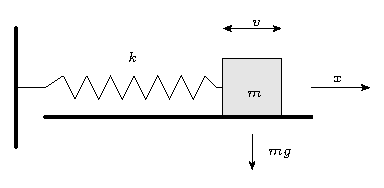
\includegraphics[width=0.5\textwidth]{task-oszillator_auf_rauer_unterlage-sketch.pdf}
  \end{figure}
  Die Anfangsbedingungen der Bewegung zur Zeit $t=0$ seien $x(0)=x_0$ und $v(0)=0$.
  \begin{atiSubtasks}
    \item{
      Lösen Sie für die ganze erste Periode der Bewegung die Differentialgleichung
      \[
        m \timeSecondDerivative{x} = -kx \mp \mu mg\ ,
      \]
      wobei das obere Vorzeichen für $v>0$ und das untere für $v<0$ gilt.
      Wie beeinflusst die Reibung die Schwingungsfrequenz?

      \begin{atiNote}
        Führen Sie die Differentialgleichung mithilfe der neuen Variablen
        \[
          \xi = x\pm \frac{\mu g}{\omega_0^2}
        \]
        auf die Gleichung des harmonischen Oszillators zurück.
      \end{atiNote}
    }
    \item{
      Geben Sie durch Verallgemeinerung Ihres Resultates $x(t)$ und $v(t)$ für die $n$-te Halbperiode für alle $n\in\setNatural$ an.
    }
    \item{
      Untersuchen Sie die Abnahme der Amplituden in aufeinanderfolgenden Perioden und zeigen Sie, dass die Maxima und Minima der Funktion $x(t)$ auf Geraden liegen.
      Bestimmen Sie die Gleichungen dieser Geraden.
      Skizzieren Sie den Verlauf der gedämpften Schwingung.
    }
  \end{atiSubtasks}
\end{atiTask}